\chapter{Projektmanagement}

In diesem Projekt werden einige Elemente der Agilen Softwareentwicklung verwendet. Was agile Softwareentwicklung ist und welche Elemente verwendet werden, wird in diesem Kapitel näher betrachtet.

\section{Agile Softwareentwicklung}

Die agile Softwareentwicklung unterscheidet sich von einer normalen Entwicklung dahingehend, dass sie den Kunden und die Funktionalität der Software in den Mittelpunkt stellt. ~\cite{F_Agile_2.1} 

\subsection{Agile Manifesto}
2001 wurden von Kent Beck und seinem Forschungsteam 12 Prinzipien im \textit{Agile Manifesto} festgelegt.~\cite{F_AgilesManifest_2.1} Folgende Auflistung enthält die Prinzipien in Kurzfassung:

\begin{itemize}
\item frühe und kontinuierliche Auslieferung von Software zur Steigerung der Kundenzufriedenheit
\item Anforderungsänderungen werden auch spät ohne Probleme angenommen
\item funktionierende Software in kurzen Abständen ausliefern
\item tägliche Zusammenarbeit von Fachexperten und Entwicklern
\item Ein Projekt erfordert motivierte Mitarbeiter, die Unterstützung, Vertrauen und das richtige Arbeitsumfeld benötigen.
\item Gespräche sind die effektivste Methode Informationen zu übermitteln
\item das wichtigste Fortschrittsmaß ist funktionierende Software
\item nachhaltige Entwicklung bedeutet ein gleichmäßiges Arbeitstempo halten zu können
\item gutes Design und technische Exzellenz sind von großer Bedeutung
\item Einfachheit ist ausschlaggebend. Sie definiert sich dadurch, die Menge nicht getaner Arbeit zu maximieren, was soviel bedeutet wie doppelte Arbeit zu vermeiden
\item Selbstorganisierte Teams entwickeln die besten Architekturen, Anforderungen und Entwürfe
\item regelmäßige Reflexion im Team zu Verbesserung der Effektivität
\end{itemize}

\subsection{Scrum}
Die Prinzipien von Kent Beck werden durch verschiedene Prozesse in einem agilen Team eingehalten. In diesem Projekt wird der agile Prozess Scrum eingesetzt. Die wichtigsten Elemente sollen im Folgenden näher betrachtet werden.

Zunächst soll die Rollenverteilung in einem Scrum Team, welches keinen typischen Projektleiter besitzt, betrachtet werden. Die erste Rolle ist die des Product Owners. Er kümmert sich darum, dass die Anforderungen an das Produkt korrekt umgesetzt werden und definiert dazu Aufgaben im sogenannten Backlog. Die zweite Rolle wird durch den Scrum Master besetzt. Dieser fungiert als Moderator der Meetings und trägt Sorge für eine gute Kommunikation innerhalb des Teams sowie nach außen hin. Des weiteren blockt er alle Störungen von außen ab, sodass das Entwicklerteam, welches die dritte Rolle darstellt, ungestört arbeiten kann. Dabei gilt als geeignete Teamgröße maximal neun Personen. Da dieses Projekt nur aus zwei Personen besteht, werden diese Rollen nicht eingehalten. Jeder nimmt jede Rolle an.

Ein Scrum Projekt ist in sogenannten Sprints organisiert, welche zwischen 1-4 Wochen dauern können. Jedoch sollte die Sprintlänge innerhalb eines Projekts konstant bleiben. Innerhalb eines Sprints wird eine abzugrenzender Teil einer Funktionalität des Produktes implementiert. Welche Aufgaben ein Sprint enthält wird im Sprint Planning unmittelbar vor Beginn des Sprints beschlossen. Am Ende eines Sprints steht das Review, indem die Implementierung überprüft wird und mit dem Product Owner besprochen wird. Zudem gibt es am Ende eines Sprints jeweils eine Retrospective, in der die Arbeitsweise des Teams überprüft wird. Während eines Sprints findet jeden Tag das sogenannte Daily statt, in dem sich das Team zu einem höchstens 15 minütigem Meeting trifft. Inhalt der Besprechung ist der gegenseitige Austausch über die erledigten Aufgaben, sowie über Probleme bei noch offenen Aufgaben. 

In diesem Projekt hat ein Sprint die Länge von 2 Wochen. Zu Beginn wird jeweils kurz geplant, welche Aufgaben zu erledigen sind und als Abschluss werden Review und Retrospective in einem durchgeführt. Ein Daily findet soweit möglich statt.

Die Aufgaben, welche der Product Owner definiert, können mit Hilfe von Kategorien geordnet werden. Dabei stellt das Epic die oberste Hierarchiestufe da. Ein Epic enthält alle Aufgaben zu einer Funktionalität des Produktes. Die Funktionalität wird dann in kleinere Abschnitte geteilt, welche innerhalb eines Sprints realisiert werden können. Diese Abschnitte werden Stories genannt. Sollte eine Story nicht innerhalb eines Sprint erledigt werden können, ist der Abschnitt zu groß definiert. Ein Story wiederum enthält die konkreten Aufgaben in Form von Tasks.~\cite{F_Scrum_2.1}

\subsection{Vor- und Nachteile agiler Softwareentwicklung}

Agile Softwareentwicklung bringt einige Vorteile mit sich. Die Implementierung ist leichter auf Veränderungen des Marktes beziehungsweise der Anforderungen anpassbar, da nicht zu Beginn ein komplettes Pflichtenheft erstellt wird und die Planung auf das Endprodukt bezogen ist, sondern eine iterative Planung vorliegt. Ein weiterer Vorteil besteht darin, dass weniger Zeit vergeht, bis erste Ergebnisse vorliegen, da funktionsorientiert programmiert wird. Durch die Definition von Aufgaben durch den Product Owner und deren Sammlung im Backlog erlangt das Team eine gewisse Flexibilität sowie einen Überblick über die zu erledigenden Aufgaben.
Allerdings ist Scrum nicht für alle Formate geeignet. Das schreiben einer Projektdokumentation gestaltet sich in einer iterativen Planung zum Beispiel eher als schwierig. Oftmals wird Scrum irrtümlich als Garant für ein gelingendes Projekt gehalten, doch es unterliegt genauso verschiedenen Deadlines und Budgetplanungen ~\cite{F_Agile_2.1}

Auf Grund der doch überwiegenden Vorteile Agiler Softwareentwicklung wurde entschieden sich an den Scrum Prozessen zu orientieren. Dabei spielt vor allen Dingen die Flexibilität in der Planung eine große Rolle. Da dieses Projekt kein Vollzeit Projekt ist, sondern neben dem normalen Studium abläuft, bringt es viele Vorteile jeden Sprint dann planen zu können, wenn er ansteht, da dann bekannt ist, wie die Gegebenheiten der Wochen sind. Da am Ende des Projektes eine Präsentation bevor steht, wirkt sich die iterative funktionsbezogene Planung ebenso positiv aus, da die Gefahr nur halbfertige Funktionen zeigen zu können nicht besteht. 


\section{Planungstool}

Zur Unterstützung der Planung des Projekts sowie zum Timetracking wird das Tool YouTrack als Cloud Lösung verwendet. In YouTrack können Epics, User Stories, Tasks, Bugs und viele weitere Arten von Issues angelegt werden. Diese können in Sprints organisiert und auf dem Agile Board angezeigt werden. Wird der Status eines Tasks auf \glqq in progress\grqq{} gestellt, startet automatisch ein Timer. Wird der Task abgeschlossen oder auf \glqq waiting \grqq{} gestellt, wird die Timer-Zeit automatisch in den Task eingetragen. YouTrack bietet dabei überall die Möglichkeit der eigenen Konfiguration.

Für das Projekt wurden folgende Epics angelegt:

\begin{itemize}
\item Projektmanagement: In diesem Epic werden alle Projektmanagement-Aufgaben angelegt.
\item Programmierung: Dieses Epic ist für alle Aufgaben für die Programmieren notwendig ist.
\item Studienarbeit schreiben: Alle Tasks die die geschriebene Studienarbeit betreffen, werden unter diesem Epic eingeordnet.
\end{itemize}

Innerhalb des Epics \textit{Projektmanagement} befinden sich die drei User Stories Youtrack Einrichtung, Dokumente erstellen und Termine planen. Das Epic \textit{Studienarbeit schreiben} beinhaltet für jedes Kapitel der Arbeit eine User Story, welche jeweils Tasks mit den zu schreibenden Abschnitten enthalten. Außerdem ist in dem Epic noch die User Story Schreibumgebung einrichten enthalten. Darin befinden sich alle Tasks betreffend der Einrichtung von Overleaf und Zotero. Im letzten Epic \textit{Programmierung} befinden sich User Stories für jedes Level welches zu gestalten ist. Dabei können dann in Tasks die verschiedenen zu erledigenden Aufgaben wie Code programmieren, Grafiken erstellen, Quiz Fragen erarbeiten und weitere festgehalten werden.

\paragraph{Timetracking}
\label{timetrackingParagraph}
Wie schon beschrieben, konnte mit Hilfe des Planungstools auch die Zeit aufgezeichnet werden, die in die jeweiligen Tasks investiert wurde. Zum Abschluss der Arbeit lässt sich nun der Time Report aus Abbildung \ref{TimeReport} erstellen. 

\begin{figure}[ht]
\centering
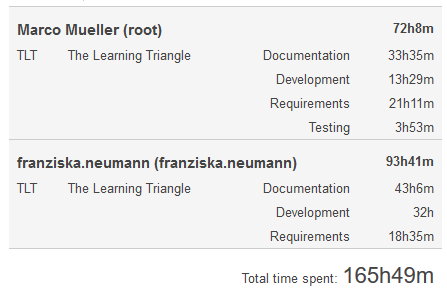
\includegraphics[scale=0.65]{bilder/TimeReport.PNG}
\caption{Time Report}
\label{TimeReport}
\end{figure}

Unterschieden wird zwischen vier Kategorien, in die Tasks unterteilt werden. \textit{Documentation} vereint dabei alle Aufgaben im Zusammenhang mit dem Schreiben der Studienarbeit, also beispielsweise das Aufsetzen eines LaTeX-Dokumentes oder der Korrekturlese. \textit{Developement} beinhaltet alle Tasks der Entwicklung, \textit{Requirements} sind nötige Vorarbeiten wie das Aneignen von Wissen. \textit{Testing} beschreibt das Testen von Anwendungen oder Ergebnissen. Diese vier Bereiche wurden so gewählt um möglichst alle Aufgabenkategorien abzudecken und dabei nicht zu viele Bereiche zu benötigen. Eine genaue Analyse mit Begründung und ein Fazit der Zeiten findet sich im Fazit in Kapitel \ref{fazitChapter}.

\section{Meilensteine und Qualitätssichernde Maßnahmen}

Ein wichtiger Bestandteil der Planung sind die Meilensteine sowie die Qualitätssichernden Maßnahmen. Meilensteine bilden dabei wichtige Zwischenschritte zur Zielerreichung. Die Qualitätssichernden Maßnahmen stellen sicher, dass diese Meilensteine auch erreicht werden. Die Planung diesbezüglich wurde in der Tabelle \ref{QSMSAnalyseBild} auf Seite \pageref{QSMSAnalyseBild} im Anhang festgehalten und jeweils zum Sprintwechsel analysiert.

Des weiteren wurde eine Meilenstein-Trend Analyse je Semester, zu sehen in Abbildungen \ref{MTA} und \ref{MTA6} auf Seite \pageref{MTA} und \pageref{MTA6} im Anhang, angelegt. Diese zeigen auf einen Blick, ob das Projekt in Verzug ist, oder ob alles in Ordnung ist. Wenn die farbigen Balken horizontal verlaufen, ist das Projekt im Zeitplan. Würde das Projekt in Verzug geraten, würden die farbigen Balken diagonal nach oben wachsen, so wie es rechts oben in der Abbildung \ref{MTA} zu sehen ist. Da es sich hier um eine Verzögerung von lediglich 3 Tagen handelt, kann gesagt werden, dass das Projekt noch im Zeitplan ist. Der unterste Meilenstein in Abbildung \ref{MTA6} wurde im Laufe des Projekts gestrichen. 

\section{Risikomanagement}
\label{riskmanagementchapter}
Ein weiterer wichtiger Bestandteil der Planung ist das Risikomanagement. Dabei geht es darum, vor Projektstart mögliche Risiken zu analysieren um ihnen im Falle eines Auftretens schnell entgegenwirken zu können. Durch Risikomanagement kann bei guter Planung das Erreichen der Projektziele abgesichert werden, sowie ein Scheitern des Projekts verhindert werden. Tritt zum Beispiel ein Problem auf, auf welches schnell reagiert werden muss, ist es vorteilhaft, wenn die Situation vorher schon bedacht wurde. Auch wenn manche Probleme nicht vollständig eliminiert werden können, so kann der Schaden doch reduziert werden.

Deshalb wurden für das Projekt folgende Problemszenarien ermittelt, deren Risikofaktor anhand Auftrittswahrscheinlichkeit und erwartetem Schaden errechnet sowie mit Gegenmaßnahmen ausgestattet. Zudem gibt es für jedes Szenario einen Verantwortlichen, welcher das Risiko im Auge behält um so möglichst frühzeitig die Gegenmaßnahmen einzuleiten. 

\paragraph{Wissensproblem - 50\% - beide}
Das größte Risiko bergen die beiden großen neuen Themengebiete AI und \textit{Educational Game}. Diese müssen für die Bearbeitung der Studienarbeit in einem gewissen Maß erarbeitet und verstanden werden. Bei schlechter Erarbeitung kann unter Umständen der Sinn des Projektes nicht erfüllt werden.

Um dem entgegen zu wirken, muss ausreichend Zeit für die Aneignung von Wissen zum Thema AI, für das Erarbeiten der Lernmethodik sowie die Durchführung eingeplant werden.

\paragraph{Klausuren - 35\% - Franziska Neumann}
Aufgrund der Erfahrung aus den letzten Jahren wird es zum Ende des Semesters oftmals stressig, da die Klausuren anstehen. Die Klausurvorbereitung nimmt dann einen großen Teil der zur Verfügung stehenden Zeit ein. Darunter kann die Studienarbeit leiden.

Deshalb sollte bei der YouTrack-Planung immer die Klausurenphase im Blick behalten werden. Große, zeitaufwendige Tasks sollten vor der stressigen Zeit erledigt werden.

\paragraph{Planung - 25\% - Marco Müller}
Ein weiteres Risiko stellt die Planung dar. Oftmals soll mehr erreicht werden als erreicht werden kann. Die unrealistische Planung kann dann aber zu Zeitproblemen führen. 

Eine Möglichkeit realistischer zu Planen stellen dabei Retrospektiven dar. In diesen wird erarbeitet, was und wie viel in welcher Zeit erledigt werden konnte. Daraufhin kann geplant werden, welche Tasks in Zukunft etwa wie viel Zeit brauchen werden.

\paragraph{Hardware - 21\% - Marco Müller}
Um ein neuronales Netz zu trainieren braucht es viel Rechenleistung. Ein Risiko ist hierbei, dass die private Rechenleistung nicht ausreicht um die Algorithmen der künstlichen Intelligenz fristgerecht zu berechnen. 

Eine Möglichkeit dieses Problem zu umgehen, ist, die \glqq Rechenleistung\grqq{} auslagern und zum Beispiel die DHBW-Computer (mit-)zu verwenden. Hierbei muss jedoch rechtzeitig ein Bedarf bei den Ansprechpartnern angemeldet werden.

\paragraph{Inkompatible Tools - 14\% - Marco Müller}
Sobald ein Projekt größer wird, werden verschiedene Tools eingesetzt. Dabei kann es passieren, dass diese nicht zusammen passen. 

Daher sollte im Vorhinein geplant werden, welche Software verwendet werden soll und geprüft werden, ob diese zusammen arbeiten. Ist dies nicht der Fall sollte nach einer alternativen Software gesucht oder ein Workaround gefunden werden.

\paragraph{Krankheit - 12\% - Franziska Neumann}
Ein weiteres Risiko besteht darin, dass ein Teammitglied krankheitsbedingt ausfällt. 

Leider kann hiergegen nicht sehr viel mehr vorbeugend unternommen werden, als darauf zu achten, ausreichend Vitamine zu essen und auf die nötige Hygiene zu achten.

\paragraph{Kommunikation - 12\% - Franziska Neumann}
Schlechte oder keine Kommunikation führt oftmals zu Missverständnissen und kann das Ziel des Projekts gefährden. Des Weiteren können Schwierigkeiten im Team ein gutes Vorankommen des Projekts verhindern.

Um dies zu verhindern sollten regelmäßige Treffen vereinbart werden und der Kontakt ständig über Email, Messenger, Telefon sowie vor Ort in der Uni gehalten werden.
